\section{RTL 仿真环境（Icarus Verilog）}

本章记录本工程\textbf{从零建立仿真环境}的完整步骤、14 个回归用例（含整机仿真）、以及仿真过程中发现的缺陷。
在此之前的第 1--19 章中，"仿真"一栏始终是"未做"。

\subsection{为什么用 Icarus Verilog}

\begin{center}
\small
\begin{tabular}{lll}
\toprule
候选方案 & 本机情况 & 结论\\
\midrule
安路 TD 6.0.3 / 5.6.5 & 只有综合与布局布线，无仿真器 & 不可用\\
ModelSim / Questa & 未安装 & 不可用\\
Vivado / Quartus & 未安装 & 不可用\\
Verilator & 未安装 & 待装\\
\textbf{Icarus Verilog 14} & 官方 Windows x64 安装包，约 26\,MB & \textbf{采用}\\
\bottomrule
\end{tabular}
\end{center}

\begin{tipbox}
\textbf{先分清这是哪种仿真。}
\begin{itemize}[leftmargin=1.6em,itemsep=1pt]
\item 本环境做的是 \textbf{RTL 行为级仿真}：\file{iverilog} 直接把工程里的 \file{.v} 源码
      编译成中间字节码（\file{.vvp}），由 \file{vvp} 调度执行；
\item 它验证 \textbf{逻辑对不对}：功能、协议、状态机、像素级行为；
\item 它\textbf{不是}门级网表仿真，\textbf{不是}时序仿真（没有门延时/布线延时/SDF 反标），
      因此不能替代综合，也不能验证建立保持时间。
\end{itemize}
\end{tipbox}

\subsection{开启仿真的步骤}

\subsubsection{第 1 步：安装 Icarus Verilog}

从 \url{https://bleyer.org/icarus/} 下载官方 Windows x64 安装包（本章使用 v14 版），
静默安装到 \file{C:/iverilog}：

\begin{lstlisting}[style=cfgcode,numbers=none]
$iv = 'iverilog-v14-20260804-x64_setup.exe'
Invoke-WebRequest -Uri "https://bleyer.org/icarus/$iv" -OutFile "$env:TEMP\$iv"
"$env:TEMP\$iv" /S                        REM 静默安装，无向导
C:\iverilog\bin\iverilog.exe -V          REM 应输出 Icarus Verilog version 14.0
C:\iverilog\bin\vvp.exe -V               REM 运行时版本
\end{lstlisting}

\begin{warnbox}
不需要仿真时，直接运行 \file{C:/iverilog/uninstall.exe} 卸载即可；
删除新增的 \file{sim/} 目录不会影响任何工程源码。
\end{warnbox}

\subsubsection{第 2 步：确认目录结构}

\begin{center}
\small
\begin{tabular}{ll}
\toprule
路径 & 内容\\
\midrule
\file{sim/run_all.ps1} & 一键编译 + 运行全部用例，按 PASS/FAIL 汇总\\
\file{sim/tb_*.v} & 14 个 testbench\\
\file{sim/ad7606_model.v} & AD7606 串行行为模型（仅仿真，不综合）\\
\file{sim/README.md} & 本目录的完整说明\\
\file{sim/_build/} & 编译产物 \file{.vvp}、波形 \file{.vcd}、导出图 \file{.raw}\\
\bottomrule
\end{tabular}
\end{center}

\subsubsection{第 3 步：一键运行}

\begin{lstlisting}[style=cfgcode,numbers=none]
powershell -ExecutionPolicy Bypass -File .\sim\run_all.ps1
REM 期望输出最后一行:  TOTAL: PASS=14  FAIL=0  SKIP=0
\end{lstlisting}

\subsubsection{第 4 步：单独跑一个用例}

\begin{lstlisting}[style=cfgcode,numbers=none]
REM 例: 只跑 AD7606 串行驱动
C:\iverilog\bin\iverilog.exe -g2005 -o sim\_build\adc.vvp sim\tb_adc_ad7606_spi.v sim\ad7606_model.v FPGA\src\adc\hal\adc_ad7606_spi.v
C:\iverilog\bin\vvp.exe -n sim\_build\adc.vvp
\end{lstlisting}

可用开关：

\begin{center}
\small
\begin{tabular}{lll}
\toprule
开关 & 作用 & 用于\\
\midrule
\sig{+vcd} & 打开波形 dump（默认关） & \file{tb_vga_timing} / \file{tb_scope_trigger}\\
\sig{-DPIX2} & 按 \sig{PIX_DIV=2} 编译 & \file{tb_vga_scope_top} 对照用例\\
\sig{+saw} / \sig{+sine} & 选择锯齿波 / 正弦波 & \file{tb_dump} 出图\\
\bottomrule
\end{tabular}
\end{center}

\subsection{回归用例清单}

\begin{center}
\small
\begin{longtable}{p{3.2cm}p{3.6cm}p{7.2cm}}
\toprule
用例 & 被测对象 & 验证内容\\
\midrule
\endhead
\file{tb_bcd} & \file{bcd.v} & 4 位 BCD：0/9/99/512/999/1000/1023（P4 修复点）\\
\file{tb_vga_timing} & \file{vga_timing.v} & de 25600\,ns、行周期 32000\,ns、行同步 3840\,ns、场同步 64000\,ns、场周期 16.8\,ms\\
\file{tb_uart_tx} & \file{uart_tx.v} & 115200 8N1、21 位时隙、0xA55A 双帧、先低字节 LSB first\\
\file{tb_uart_rx} & \file{uart_rx.v} & 按位注入 8N1，0x55/0xAA/0x00/0xFF/0x5A 逐字节还原\\
\file{tb_cmd_chain} & \file{uart_rx}+\file{scope_cmd}+\file{adc_cmd} & 真串口喂 ASCII：T/R/A/L/E/S/M/C/P/H 与 R/O/S/K/N 全部命中；未知命令与小写不产生写\\
\file{tb_scope_capture} & \file{scope_capture.v} & 触发状态机、\sig{rd_base}=触发地址$-$pre\_trig、DONE 停写、auto 不进 FILL\\
\file{tb_scope_trigger} & \file{vga_scope_top.v} & 触发锁相（缓冲相位 0 个不符点）、关触发后相位漂移、滚动最右列最新\\
\file{tb_adc_ad7606_spi} & \file{adc_ad7606_spi.v} & 复位脉冲、64 个 SCLK、4 路 16bit 补码逐位还原（含 0x0001/0x8000）\\
\file{tb_adc_ad7606_top} & \file{adc_ad7606_top.v} & CSR 读写、补码$\to$偏移二进制$\to$取高 10 位（0x1234$\to$584 等）\\
\file{tb_vga_scope_top} & \file{vga_scope_top.v} & 整屏：307200 像素/帧、颜色分布、y=223/224 整行、斜坡铺满 0..447\\
\file{tb_vga_scope_top_pix2} & 同上（\sig{-DPIX2}） & \sig{PIX_DIV=2} 对照，两个配置产出图像必须一致\\
\file{tb_vga_test_top} & \file{vga_test_top.v} & 屏幕自检 5 幅画面：连抓 5 帧按内容分类，要求彩条/灰阶/棋盘/边框/文字全部出现\\
\file{tb_sparkroad_top} & \file{sparkroad_scope_top.v} & 整机：ADC 复位与 locked、串口 \sig{T0000} 生效、CONVST 起振、整帧 307200 像素且波形随输入变化、数码管扫描、串口 TX 有起始位\\
\bottomrule
\end{longtable}
\end{center}

\subsection{AD7606 行为模型}

\file{ad7606_model.v} 按数据手册串行读时序建模，\textbf{只用于仿真、不参与综合}：

\begin{center}
\small
\begin{tabular}{ll}
\toprule
事件 & 模型行为\\
\midrule
CONVST 上升沿 & 锁存 ch1..ch4，BUSY 拉高\\
BUSY & 维持 \sig{CONV_CLK} 个 clk 后拉低（默认 60，模拟转换时间）\\
CS 下降沿 & 位指针归零，开始一帧\\
SCLK 下降沿 & 输出下一位；\textbf{第 1 个下降沿输出 ch1 的 D15}\\
SCLK 上升沿 & 主机采样（数据在下降沿已稳定）\\
一帧 64 位 & ch1..ch4 各 16\,bit，MSB first\\
\bottomrule
\end{tabular}
\end{center}

\begin{warnbox}
\sig{DOUTA} 必须用 \sig{always @(negedge sclk)} 事件驱动，\textbf{不能用 clk 打拍}：
\sig{sdiv=1}（半周期只有 1 个 clk）时打拍版本会晚一拍，整帧错位 16 位。
\end{warnbox}

\subsection{整屏仿真与出图}

\file{tb_dump.v} 把 \file{vga_scope_top} 的\textbf{真实输出像素}导出：等一次捕获完成
（\sig{state=DONE}，缓冲冻结）后，按像素把 \sig{vga_rgb} 写成每像素 2 字节的
\file{frame.raw}，再用 Python/Pillow 转成 PNG。

\begin{lstlisting}[style=cfgcode,numbers=none]
cd sim\_build
C:\iverilog\bin\vvp.exe -n .\dump.vvp +sine    REM +saw / 不带开关=方波
python raw2png.py frame_sine.raw ..\scope_wave_sine.png
\end{lstlisting}

三幅图均来自上述流程（\textbf{不是数学示意，是仿真输出的原样像素}），
对比第 15 章的 \file{preview_640x480.png} 是用 Python 复现的渲染数学。

\begin{figure}[htbp]
\centering
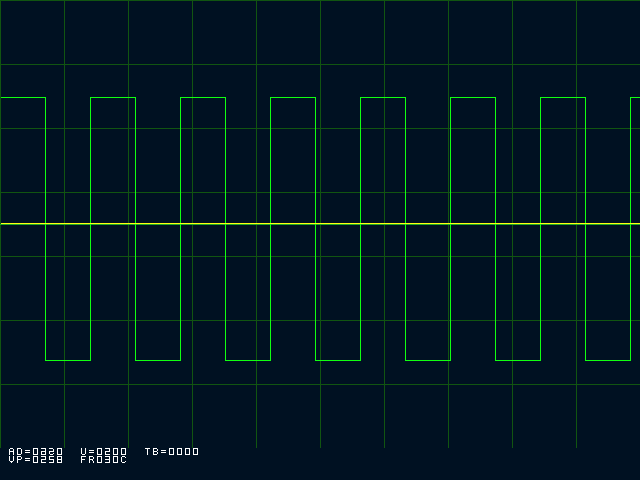
\includegraphics[width=0.72\linewidth]{../sim/scope_wave_square.png}
\caption{方波输入（周期 90 采样点，800/200）：触发锁定后波形稳定，CH1 为黄色直线}
\label{fig:sim-square}
\end{figure}

\begin{figure}[htbp]
\centering
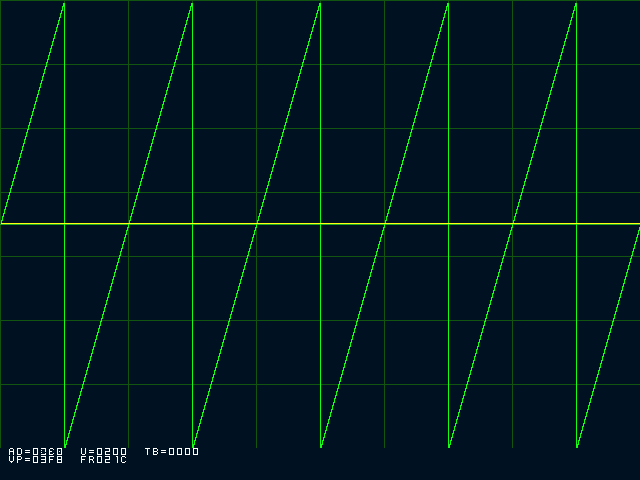
\includegraphics[width=0.72\linewidth]{../sim/scope_wave_saw.png}
\caption{锯齿波输入（周期 128 采样点，0$\to$1016）：可见 5 个周期与陡峭回扫沿}
\label{fig:sim-saw}
\end{figure}

\begin{figure}[htbp]
\centering
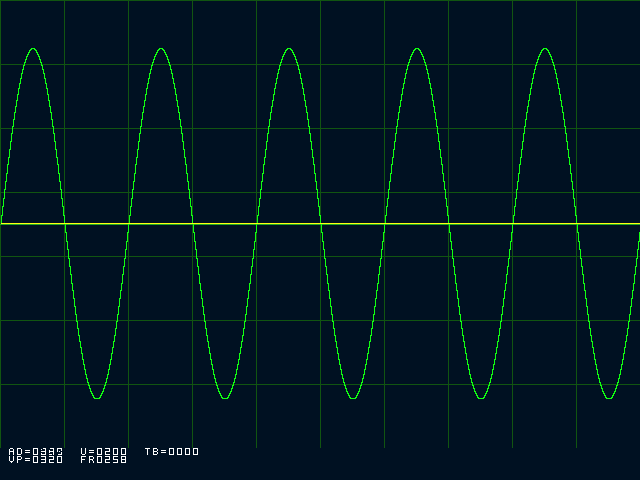
\includegraphics[width=0.72\linewidth]{../sim/scope_wave_sine.png}
\caption{正弦波输入（128 点查表，中心 512、幅度 400）：波形平滑，纵轴映射正确}
\label{fig:sim-sine}
\end{figure}

\subsubsection{整机仿真}

\file{tb_sparkroad_top.v} 仿真的是\textbf{出比特流的那个顶层本身}：24\,MHz 时钟、
\file{ad7606_model} 接在 AD7606 引脚上、串口喂命令、抓一整帧 VGA。它一次跑通
「ADC $\to$ HAL $\to$ 采集/触发/测量 $\to$ 图层合成 $\to$ RGB888 $\to$ VGA 引脚」
整条链路，并同时检查数码管扫描与串口发送。

\begin{figure}[htbp]
\centering
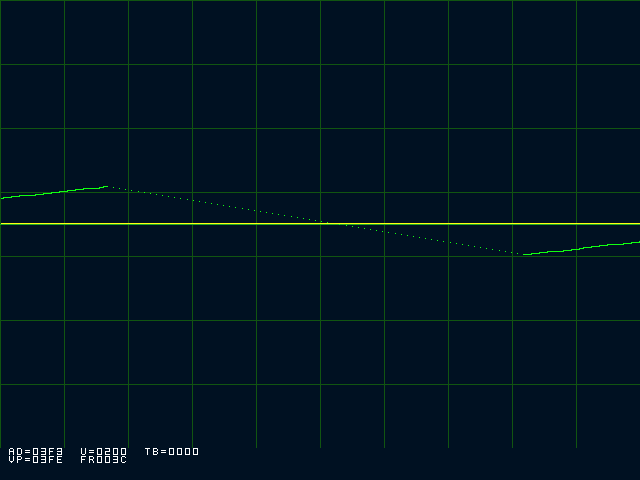
\includegraphics[width=0.72\linewidth]{../sim/scope_top_full.png}
\caption{整机仿真输出的一帧（\file{sparkroad_scope_top}）：ADC 模型输入斜坡。
波形呈"阶梯虚线"是\textbf{激励特性}（模型 4 个通道同值、采样率约为像素时钟的 1/500），
不是渲染缺陷}
\label{fig:sim-top}
\end{figure}

\subsubsection{PLL 空壳}

\file{gowin_pll_shell.v} 用行为代码替代高云原语 \sig{PLLA}（50\,MHz 分 6.25\,MHz 两路）。
但全仓检索确认：\textbf{两个总顶层都没有例化 Gowin\_PLL}——\file{adda.v} 第 385、412 行
附近两处例化都是注释掉的，1\,kHz 时钟由 \file{divider} 提供；\file{fifo_top} 同样未例化。
因此\textbf{仿真总顶层并不需要 PLL 空壳}；该文件是为以后启用 PLL
（例如 24\,MHz 换 25.175\,MHz 像素时钟）预留的，编译时用它替代 \file{gowin_pll.v} 即可。

\subsection{仿真发现的问题}

\begin{longtable}{p{0.6cm}p{3.4cm}p{9.6cm}}
\toprule
编号 & 位置 & 结论\\
\midrule
\endhead
S1 & \file{vga_scope_top.v} & \sig{PIX_DIV=1}（SparkRoad 实际配置）时每行\textbf{最后一列 x=639 恒为背景色}，
网格/文字左移 1 像素。根因：网格/文字是组合逻辑（1 拍），波形要过 BSRAM 同步读（2 拍），
而 \sig{de} 延迟 2 拍；\sig{PIX_DIV=2} 时 1 拍差被吸收，\sig{PIX_DIV=1} 时暴露。
\textbf{已修复}：图层前加 \sig{px_d/py_d/de_d} 打一拍。\\
S2 & \file{adc_ad7606_spi.v} & CONVST 宽度实为 \sig{CONV_CYC+1} 拍、CS 低电平为
\sig{64*2*sdiv+1} 拍（FSM 打拍所致），功能无害但按时序预算会差一拍。\\
S3 & \file{vga_timing.v} & 端口注释写 \sig{px/py} 范围 0..H\_VIS$-$1，实际是 0..799/0..524；
消隐期照样在数，\textbf{新图层若直接用 px 而不经 de 屏蔽就会算错}。\\
S4 & \file{scope_cmd.v}/\file{adc_cmd.v} & \sig{R}、\sig{S} 被两个解析器同时解释
（示波器 + ADC 各写各的），上板调参时一次按键会改两处；命令字母大小写敏感。\\
\bottomrule
\end{longtable}

\subsubsection{S1 的修复与重综合}

修复：在三个图层（网格/文字/波形）之前插入 \sig{px_d/py_d/de_d} 打一拍的对齐寄存器，
\sig{raddr} 仍用未延迟的 \sig{px} 以配合 BSRAM 的 1 拍读延迟。
修复后 \sig{PIX_DIV=1} 与 \sig{PIX_DIV=2} 的整帧颜色计数逐项相同。

\begin{center}
\small
\begin{tabular}{lrr}
\toprule
项目 & 修复前 \file{scope_eg4_60} & 修复后 \file{scope_eg4_61}\\
\midrule
LUT & 1632 / 19600 & 1645 / 19600\\
寄存器 & 832 & \textbf{857}（+25 = 12 px\_d + 12 py\_d + 1 de\_d）\\
DSP / BRAM / PAD & 6 / 4 / 51 & 6 / 4 / 51\\
Setup slack @24\,MHz & +20.485\,ns & \textbf{+21.964\,ns}\\
时序错误 & 0 & \textbf{0 setup / 0 hold}\\
比特流 & 634296\,B & 634296\,B\\
\bottomrule
\end{tabular}
\end{center}

流程脚本：\file{FPGA_TD/full_flow61.tcl}（与 \file{full_flow60.tcl} 仅工程名不同，
不覆盖已归档的 60 版）；比特流在
\file{FPGA_TD/scope_eg4_61_Runs/best_result/scope_eg4_61.bit}。

\begin{warnbox}
\textbf{改名后的比特流才与当前源码一致。}旧文件
\file{FPGA_TD/eg4/bit/scope_eg4_60.bit} 对应修复前的 RTL，上板请改用 61 版。
\end{warnbox}

\subsection{覆盖矩阵}

\begin{center}
\small
\begin{tabular}{lll}
\toprule
层 & 模块 & 状态\\
\midrule
HAL & \file{vga_timing}、\file{vram_sdp}、\file{font_rom} & 已覆盖\\
ABS & \file{grid_layer}、\file{trace_layer}、\file{text_layer}、\file{compositor} & 已覆盖\\
APP & \file{scope_capture}、\file{scope_meas}、\file{scope_app}、\file{scope_ui} & 已覆盖\\
APP & \file{scope_cmd}、\file{adc_cmd} & 已覆盖（端到端）\\
ADC & \file{adc_ad7606_spi}、\file{adc_ad7606_top}、\file{adc_cfg}、\file{adc_norm} & 已覆盖\\
其它 & \file{bcd}、\file{uart_tx}、\file{uart_rx} & 已覆盖\\
\midrule
未覆盖 & \file{vga_test_top}（自检图案） & 无依赖，最容易补\\
未覆盖 & \file{adda_scope_top}、\file{sparkroad_scope_top} & 缺 PLL 空壳模型\\
不可仿真 & \file{gowin_pll.v}（PLLA 原语）、\file{fifo_top.v}（IEEE 1735 加密） & 需行为模型替代\\
\bottomrule
\end{tabular}
\end{center}

\subsection{约定}

\begin{itemize}[leftmargin=2em,itemsep=1pt]
\item 每个用例输出一行 \sig{[tb_xxx] PASS} 或 \sig{[tb_xxx] FAIL}，脚本按关键字判定；
\item 新增用例：写 \file{sim/tb_*.v}，在 \file{run_all.ps1} 的 \$cases 里加一行
      （\$srcs 相对 \file{FPGA/src}，\$local 相对 \file{sim/}）；
\item 只读工程源码，仿真产物全部落在 \file{sim/_build/}；
\item \textbf{仿真通过不等于可以上板}：最终仍需综合 + 实板验证。
\end{itemize}
